\documentclass[12pt,a4paper]{article}

\usepackage[utf8]{inputenc}
\usepackage[T5]{fontenc}
\usepackage[vietnamese]{babel}
\usepackage{amsmath,amssymb}
\usepackage{graphicx}
\usepackage{booktabs}
\usepackage{hyperref}
\usepackage{geometry}
\usepackage{float}
\usepackage{caption}
\usepackage{subcaption}
\usepackage{array}
\usepackage{multirow}
\usepackage{listings}
\usepackage{xcolor}
\usepackage{enumitem}
\usepackage{parskip}
\usepackage{fancyhdr}

\geometry{top=2.5cm, bottom=2.5cm, left=3cm, right=2.5cm}

\hypersetup{colorlinks=true, linkcolor=blue, urlcolor=cyan}

\lstset{
    basicstyle=\footnotesize\ttfamily,
    breaklines=true,
    backgroundcolor=\color{gray!8},
    frame=single,
    language=Python,
    keywordstyle=\color{blue},
    commentstyle=\color{green!60!black},
    stringstyle=\color{orange}
}

\pagestyle{fancy}
\fancyhf{}
\rhead{Deep Learning for Time Series Forecasting}
\lhead{Báo cáo Thực hành}
\cfoot{\thepage}

% ============================================================
\begin{document}

\begin{titlepage}
    \centering
    \vspace*{2cm}
    {\Large\textbf{ĐẠI HỌC KINH TẾ -- LUẬT}}\\[0.3em]
    {\large KHOA HỆ THỐNG THÔNG TIN}\\[2cm]
    \rule{\linewidth}{0.5mm}\\[0.4cm]
    {\LARGE\textbf{BÁO CÁO THỰC HÀNH}}\\[0.3em]
    {\Large Deep Learning cho Dự báo Chuỗi Thời gian}\\[0.2em]
    {\large MLP, CNN và LSTM Networks}\\
    \rule{\linewidth}{0.5mm}\\[2cm]
    \begin{tabular}{rl}
        \textbf{Sinh viên:} & Phạm Trần Thanh Tài \\[0.3em]
        \textbf{MSSV:}      & K234161852 \\[0.3em]
        \textbf{Môn học:}   & Deep Learning for Time Series \\[0.3em]
        \textbf{Ngày nộp:}  & Tháng 6, 2026 \\
    \end{tabular}
    \vfill
    {\large TP. Hồ Chí Minh, 2026}
\end{titlepage}

\tableofcontents
\newpage

% ============================================================
\section{Phần 0 --- Khởi động: Từ Chuỗi thành Dữ liệu Huấn luyện (5\%)}

\subsection{(a) Công thức số lượng mẫu one-step}

Với một chuỗi có độ dài $N$ và cửa sổ trượt $n\_steps$, mỗi mẫu gồm $n\_steps$ giá trị đầu vào và 1 giá trị mục tiêu kế tiếp. Cửa sổ đầu tiên chiếm vị trí $[0,\, n\_steps-1]$ và dự đoán vị trí $n\_steps$; cửa sổ cuối cùng chiếm $[N-n\_steps-1,\, N-2]$ và dự đoán $N-1$. Suy ra:

\[
\boxed{\text{Số mẫu} = N - n\_steps}
\]

\textbf{Xác minh thực nghiệm:} Chạy \texttt{python dl\_time\_series\_practice.py data} với chuỗi $[10, 20, 30, 40, 50, 60, 70]$ ($N=7$, $n\_steps=3$): công thức cho $7-3=4$ mẫu, đầu ra xác nhận:

\begin{center}
\begin{tabular}{ccc}
\toprule
\textbf{X (đầu vào)} & & \textbf{y (mục tiêu)} \\
\midrule
$[10,\ 20,\ 30]$ & $\rightarrow$ & $40$ \\
$[20,\ 30,\ 40]$ & $\rightarrow$ & $50$ \\
$[30,\ 40,\ 50]$ & $\rightarrow$ & $60$ \\
$[40,\ 50,\ 60]$ & $\rightarrow$ & $70$ \\
\bottomrule
\end{tabular}
\end{center}

\subsection{(b) Phân biệt One-step và Multi-step Windowing}

\textbf{One-step:} Mỗi cửa sổ dự đoán duy nhất một giá trị kế tiếp. Chuỗi $N$ điểm tạo ra $N - n\_steps$ mẫu với $y \in \mathbb{R}$.

\textbf{Multi-step:} Mỗi cửa sổ dự đoán $n\_out$ giá trị liên tiếp. Số mẫu là $N - n\_steps - n\_out + 1$, với $y \in \mathbb{R}^{n\_out}$. Mô hình phải cam kết với toàn bộ chân trời dự báo trong một lần suy luận.

\textbf{Ví dụ thực tế:}
\begin{itemize}[leftmargin=*]
    \item \textit{One-step:} Dự báo lượng điện tiêu thụ giờ tiếp theo, cập nhật liên tục theo thời gian thực.
    \item \textit{Multi-step:} Dự báo thời tiết 7 ngày tới để lên lịch sự kiện ngoài trời --- cần 7 giá trị đồng thời trước khi sự kiện diễn ra.
\end{itemize}

% ============================================================
\section{Phần 1 --- Phân tích Khám phá Dữ liệu (15\%)}

\subsection{(a) Xu hướng và Tính mùa vụ}

\subsubsection*{Bộ dữ liệu Airline (Hành khách hàng không quốc tế, 1949--1960)}

\begin{figure}[H]
    \centering
    \begin{subfigure}[b]{0.48\textwidth}
        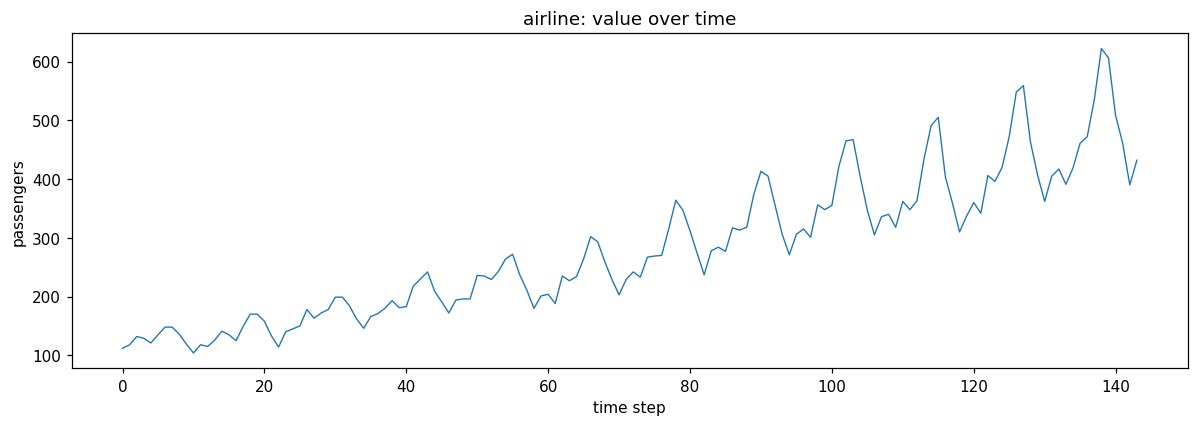
\includegraphics[width=\textwidth]{eda_outputs/airline_01_series.png}
        \caption{Chuỗi gốc}
    \end{subfigure}
    \hfill
    \begin{subfigure}[b]{0.48\textwidth}
        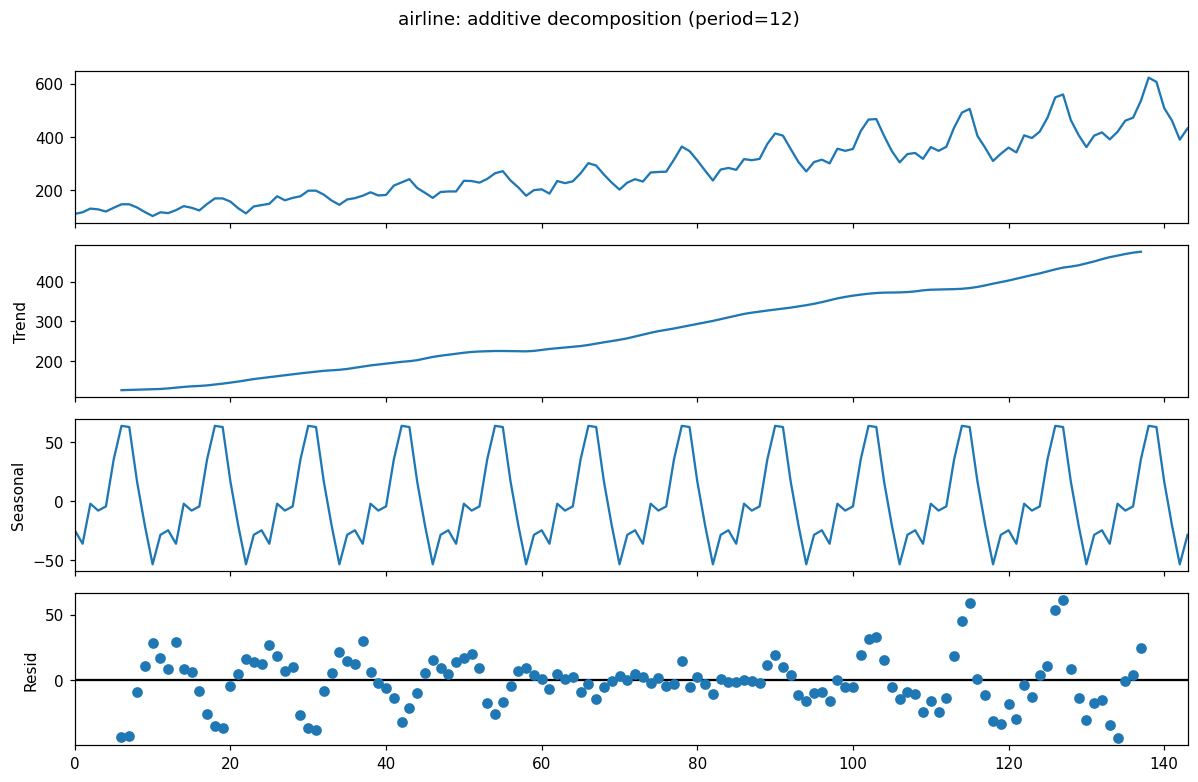
\includegraphics[width=\textwidth]{eda_outputs/airline_04_decomposition.png}
        \caption{Phân rã mùa vụ (period=12)}
    \end{subfigure}
    \caption{Dữ liệu Airline Passengers: trực quan và phân rã}
\end{figure}

\begin{itemize}
    \item \textbf{Xu hướng (Trend):} Tăng trưởng mạnh và liên tục, từ $\sim$100 lên $\sim$600 nghìn hành khách trong 12 năm. Trung bình nửa sau lớn hơn nửa đầu $+194.79$, xác nhận xu hướng rõ nét.
    \item \textbf{Tính mùa vụ:} Chu kỳ \textbf{12 tháng} (1 năm). Số hành khách tăng vào tháng 7--8 (hè Bắc bán cầu -- mùa du lịch) và giảm vào cuối năm. Chu kỳ 12 tháng đúng với thực tế: hành vi du lịch hàng không phụ thuộc theo mùa.
    \item \textbf{Tính mùa vụ nhân tính:} Biên độ dao động mùa vụ tăng theo thời gian (khi mức tăng xu hướng tăng, dao động cũng tăng) --- đây là \textit{multiplicative seasonality}.
\end{itemize}

\subsubsection*{Bộ dữ liệu Temps (Nhiệt độ tối thiểu hàng ngày, Melbourne, 1981--1990)}

\begin{figure}[H]
    \centering
    \begin{subfigure}[b]{0.48\textwidth}
        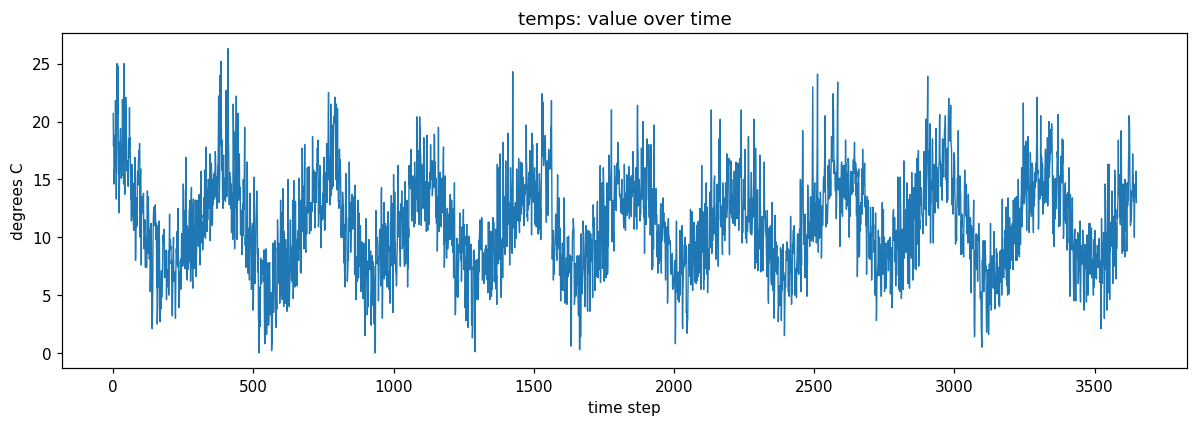
\includegraphics[width=\textwidth]{eda_outputs/temps_01_series.png}
        \caption{Chuỗi gốc}
    \end{subfigure}
    \hfill
    \begin{subfigure}[b]{0.48\textwidth}
        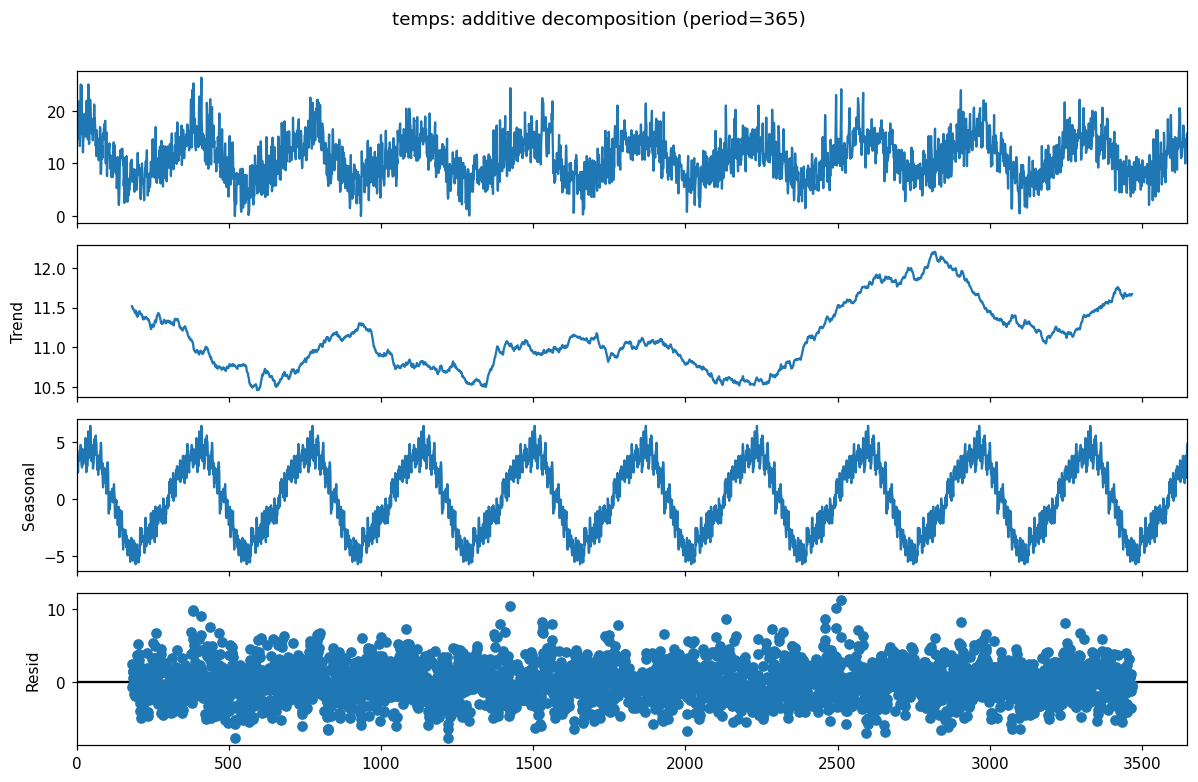
\includegraphics[width=\textwidth]{eda_outputs/temps_04_decomposition.png}
        \caption{Phân rã mùa vụ (period=365)}
    \end{subfigure}
    \caption{Dữ liệu Temps: trực quan và phân rã}
\end{figure}

\begin{itemize}
    \item \textbf{Xu hướng:} Gần như không tồn tại. Chênh lệch trung bình nửa sau so với nửa đầu chỉ $+0.27^\circ$C trong 10 năm.
    \item \textbf{Tính mùa vụ:} Chu kỳ \textbf{365 ngày} (1 năm). Nhiệt độ thấp vào mùa đông Úc (tháng 6--8, $\sim$5--8$^\circ$C) và cao vào mùa hè (tháng 12--2, $\sim$15--20$^\circ$C). Melbourne ở Nam bán cầu nên mùa đông rơi vào giữa năm --- đúng với thực tế địa lý.
    \item \textbf{Tính mùa vụ cộng tính:} Biên độ dao động ổn định theo thời gian, trái ngược với airline.
\end{itemize}

\subsection{(b) Kiểm định Tính dừng (ADF Test)}

\begin{table}[H]
\centering
\caption{Kết quả kiểm định ADF}
\begin{tabular}{llccp{4.5cm}}
\toprule
\textbf{Dataset} & \textbf{Biến thể} & \textbf{ADF Stat} & \textbf{p-value} & \textbf{Kết luận} \\
\midrule
Airline & Gốc            & $+0.8154$ & $0.9919$ & Không dừng \\
Airline & Sai phân bậc 1 & $-2.8293$ & $0.0542$ & Không dừng \\
\midrule
Temps   & Gốc            & $-4.4448$ & $0.0002$ & \textbf{Dừng} \\
Temps   & Sai phân bậc 1 & $-18.028$ & $<0.0001$& \textbf{Dừng} \\
\bottomrule
\end{tabular}
\end{table}

\begin{itemize}
    \item \textbf{Temps} dừng ngay từ đầu ($p = 0.0002 < 0.05$): không có xu hướng dài hạn, phương sai ổn định.
    \item \textbf{Airline} vẫn không dừng sau sai phân bậc 1 ($p = 0.054 > 0.05$). \textit{Lý do:} Sai phân bậc 1 chỉ loại bỏ xu hướng tuyến tính. Tuy nhiên, airline còn có \textbf{tính mùa vụ nhân tính với biên độ tăng dần} mà sai phân đơn không xóa được. Biểu đồ phân rã vẫn còn thành phần seasonal rõ ràng sau differencing. Để đạt tính dừng hoàn toàn cần thêm: sai phân mùa vụ tại lag 12, hoặc biến đổi logarithm trước.
\end{itemize}

\subsection{(c) Phân phối}

\begin{figure}[H]
    \centering
    \begin{subfigure}[b]{0.48\textwidth}
        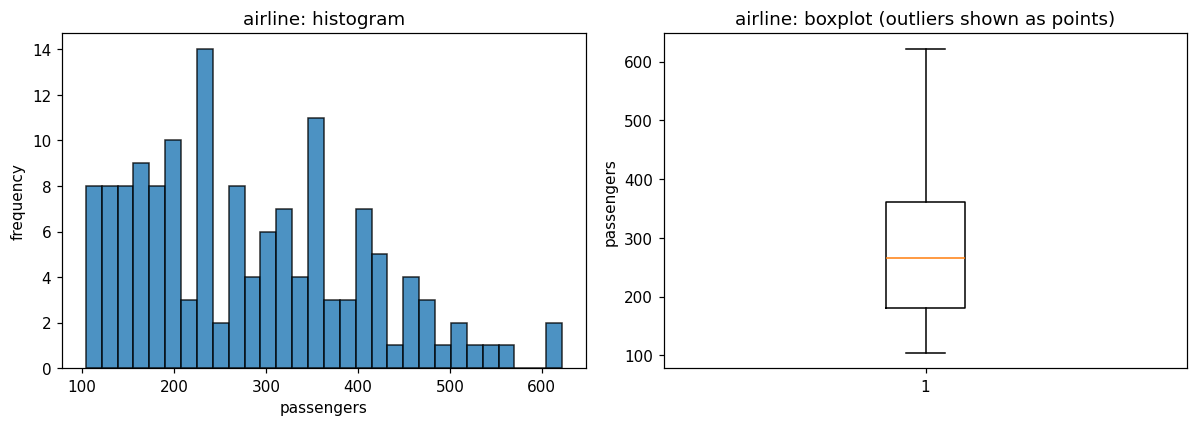
\includegraphics[width=\textwidth]{eda_outputs/airline_02_distribution.png}
        \caption{Phân phối Airline}
    \end{subfigure}
    \hfill
    \begin{subfigure}[b]{0.48\textwidth}
        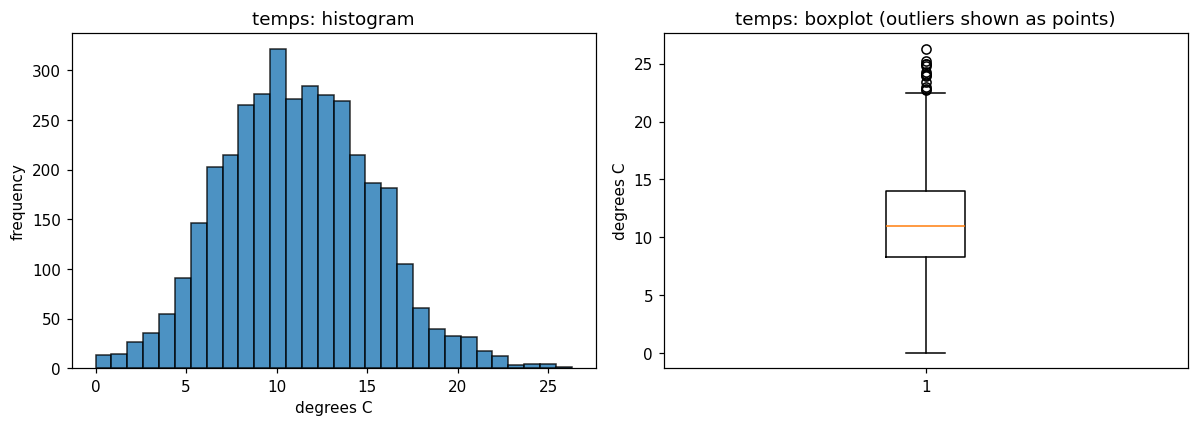
\includegraphics[width=\textwidth]{eda_outputs/temps_02_distribution.png}
        \caption{Phân phối Temps}
    \end{subfigure}
    \caption{Histogram và Boxplot}
\end{figure}

\begin{itemize}
    \item \textbf{Airline:} Phân phối lệch phải mạnh (right-skewed) do xu hướng tăng trưởng. Boxplot không có outliers thực sự --- các giá trị cao là hệ quả tự nhiên của xu hướng. Không đối xứng.
    \item \textbf{Temps:} Phân phối xấp xỉ đối xứng quanh median $11^\circ$C ($\approx$ chuẩn), với đuôi phải nhẹ. Boxplot cho thấy một vài điểm outlier ở đuôi trên (ngày đặc biệt nóng).
\end{itemize}

\subsection{(d) Chọn kích thước cửa sổ từ PACF}

\begin{figure}[H]
    \centering
    \begin{subfigure}[b]{0.48\textwidth}
        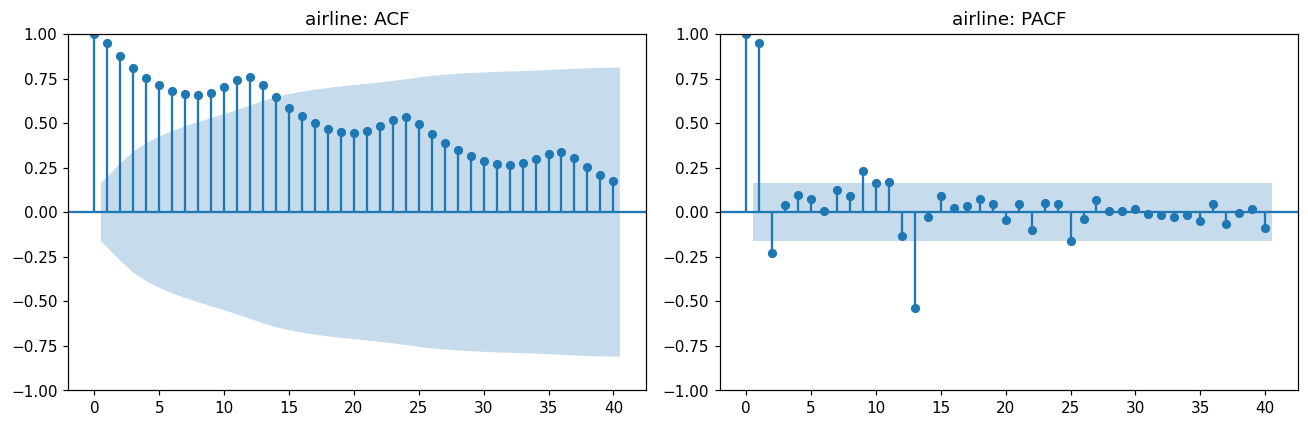
\includegraphics[width=\textwidth]{eda_outputs/airline_05_acf_pacf.png}
        \caption{ACF/PACF Airline}
    \end{subfigure}
    \hfill
    \begin{subfigure}[b]{0.48\textwidth}
        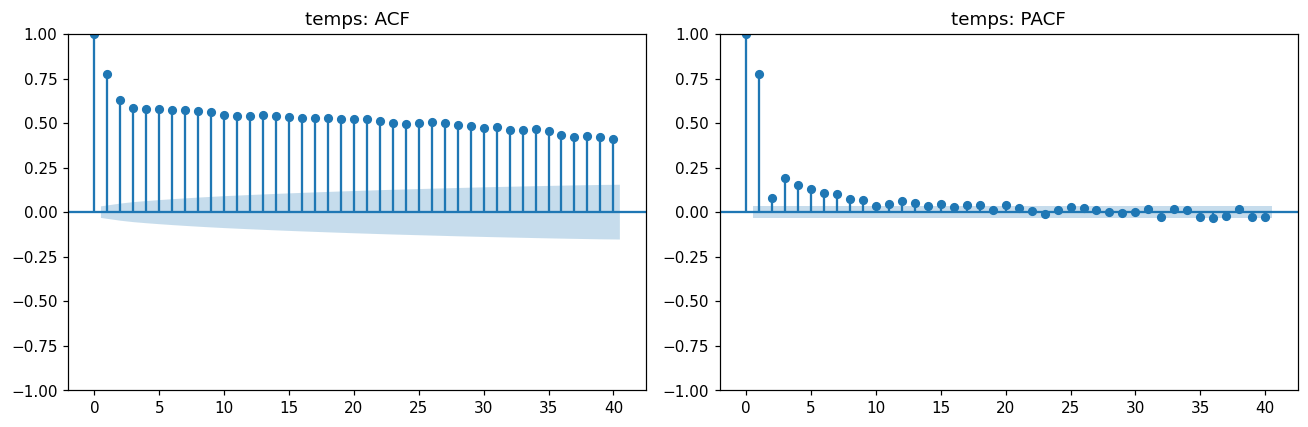
\includegraphics[width=\textwidth]{eda_outputs/temps_05_acf_pacf.png}
        \caption{ACF/PACF Temps}
    \end{subfigure}
    \caption{Biểu đồ ACF và PACF (lags=40)}
\end{figure}

\begin{itemize}
    \item \textbf{Airline:} PACF có spike đáng kể tại lag 1, lag 2, và lag 12 (mùa vụ hàng năm). Gợi ý $n\_steps = 12$ để mô hình ``nhìn thấy'' đúng một chu kỳ mùa vụ đầy đủ.
    \item \textbf{Temps:} PACF có spike đáng kể tại lag 1--7, sau đó suy giảm nhanh. Gợi ý $n\_steps \in [7, 14]$ --- đủ nắm bắt phụ thuộc ngắn hạn trong 1--2 tuần.
\end{itemize}

Dự đoán từ PACF sẽ được kiểm tra tại \textbf{Phần 4.4}: kết quả thực nghiệm xác nhận $n\_steps = 14$ là tốt nhất.

% ============================================================
\section{Phần 2 --- Demo Mô hình Tổng hợp (10\%)}

\subsection{(a) RMSE từng mô hình}

Chuỗi tổng hợp: $y(t) = 10\sin(2\pi t/25) + 0.05t + \epsilon_t$, $\epsilon_t \sim \mathcal{N}(0,1)$, $N=400$, $n\_steps=20$.

\begin{table}[H]
\centering
\caption{RMSE kiểm thử trên chuỗi tổng hợp (SEED=42)}
\begin{tabular}{lcc}
\toprule
\textbf{Mô hình} & \textbf{RMSE} & \textbf{Ghi chú} \\
\midrule
MLP                   & 1.452 & Demo riêng \\
CNN                   & 1.363 & Demo riêng \\
LSTM Vanilla          & 1.284 & Demo riêng \\
LSTM Stacked (2 lớp)  & 1.366 & Demo riêng \\
LSTM Bidirectional    & 2.353 & Demo riêng \\
\midrule
\multicolumn{3}{c}{\textit{So sánh trực tiếp trên cùng split (demo\_compare)}} \\
\midrule
MLP         & 1.300 & \\
LSTM Vanilla& 1.316 & \\
CNN         & 1.531 & \\
\bottomrule
\end{tabular}
\end{table}

\subsection{(b) Sàn RMSE lý thuyết}

Nhiễu $\epsilon_t \sim \mathcal{N}(0, 1)$ có $\sigma = 1.0$. Bất kỳ mô hình hoàn hảo nào cũng không thể dự đoán thành phần ngẫu nhiên, nên:
\[
\text{RMSE}_{\min} \approx \sigma_\epsilon = 1.0
\]
Kết quả: LSTM Vanilla đạt $1.284$, MLP đạt $1.300$ --- gần sàn lý thuyết. Tất cả mô hình đã học được phần lớn cấu trúc xác định của chuỗi.

\subsection{(c) Độ nhạy theo Random Seed}

\begin{table}[H]
\centering
\caption{RMSE theo SEED khác nhau (\texttt{demo\_compare}, n\_steps=20)}
\begin{tabular}{cccc}
\toprule
\textbf{SEED} & \textbf{MLP} & \textbf{CNN} & \textbf{LSTM} \\
\midrule
42  & 1.300 & 1.531 & 1.316 \\
0   & 1.217 & 1.317 & 1.324 \\
7   & 1.310 & 1.513 & 1.904 \\
123 & 1.246 & 1.487 & 1.329 \\
\bottomrule
\end{tabular}
\end{table}

\textbf{Nhận xét:} Thứ hạng thay đổi đáng kể: ở SEED=42 CNN tệ nhất, ở SEED=0 CNN đứng giữa. LSTM dao động nhiều nhất (1.284 đến 2.353). \textbf{Kết luận: không thể tuyên bố một kiến trúc ``tốt nhất'' từ một lần chạy duy nhất.} Đánh giá công bằng cần chạy nhiều lần với seed ngẫu nhiên và báo cáo mean $\pm$ std.

% ============================================================
\section{Phần 3 --- Dữ liệu Thực, Scaling, và Baseline (10\%)}

\subsection{(a) RMSE thực tế so với Baseline}

\begin{table}[H]
\centering
\caption{So sánh RMSE --- Airline (đơn vị: nghìn hành khách)}
\begin{tabular}{lcr}
\toprule
\textbf{Mô hình} & \textbf{RMSE} & \textbf{Cải thiện vs Naive} \\
\midrule
Naive Baseline & 53.355 & ---       \\
CNN            & 19.677 & $-63.1\%$ \\
MLP            & 21.300 & $-60.1\%$ \\
LSTM           & 39.541 & $-25.9\%$ \\
\bottomrule
\end{tabular}
\end{table}

\begin{table}[H]
\centering
\caption{So sánh RMSE --- Temps (đơn vị: $^\circ$C)}
\begin{tabular}{lcr}
\toprule
\textbf{Mô hình} & \textbf{RMSE} & \textbf{Cải thiện vs Naive} \\
\midrule
Naive Baseline & 2.481 & ---       \\
\textbf{LSTM}  & \textbf{2.207} & $\mathbf{-11.0\%}$ \\
MLP            & 2.610 & $+5.2\%$ (kém hơn) \\
CNN            & 2.711 & $+9.3\%$ (kém hơn) \\
\bottomrule
\end{tabular}
\end{table}

\begin{itemize}
    \item \textbf{Airline:} Tất cả mô hình vượt baseline rõ ràng. CNN và MLP giảm RMSE trên $60\%$.
    \item \textbf{Temps:} Chỉ LSTM vượt baseline ($-11\%$). MLP và CNN \textit{tệ hơn} cả naive.
\end{itemize}

\subsection{(b) Tại sao Airline dễ còn Temps khó?}

\begin{itemize}
    \item \textbf{Airline có xu hướng mạnh + mùa vụ rõ:} Khi chuỗi liên tục tăng, persistence baseline (``hôm nay = hôm qua'') mắc sai số tích lũy lớn. Mô hình chỉ cần học xu hướng và chu kỳ đã vượt xa baseline.
    \item \textbf{Temps đã dừng + nhiều nhiễu:} Chuỗi nhiệt độ không có xu hướng; nhiệt độ ngày mai thực sự rất gần ngày hôm nay ($\sigma \approx 4.07^\circ$C, persistence RMSE chỉ $2.48^\circ$C). ``Dư địa'' cải thiện rất nhỏ. Tỉ lệ nhiễu/tín hiệu cao khiến mô hình khó học hơn tín hiệu thực sự.
\end{itemize}

\subsection{(c) Tại sao Fit Scaler trên Train và Inverse-transform?}

\textbf{(i) Fit scaler chỉ trên tập train:}
Nếu fit scaler trên toàn bộ dữ liệu (bao gồm test), thống kê min/max của tương lai sẽ ``rò rỉ'' vào huấn luyện --- \textit{data leakage}. Mô hình học trong không gian đặc trưng được xây dựng bởi thông tin không thể có trong thực tế. Kết quả đánh giá sẽ lạc quan giả tạo (\textit{optimistically biased}).

\textbf{(ii) Inverse-transform trước khi tính RMSE:}
Dự đoán nằm trong $[0, 1]$ (scaled) --- đây là đơn vị vô nghĩa. ``RMSE = 0.05'' không truyền đạt thông tin thực tế. Sau inverse-transform, ``RMSE = 21.3 nghìn hành khách'' mới có ý nghĩa để so sánh với baseline và đánh giá tác động kinh doanh. Thiếu bước này đồng nghĩa với việc báo cáo con số không thể hiểu hoặc so sánh.

% ============================================================
\section{Phần 4 --- Triển khai Các Bài Tập (40\%)}

\subsection{Task 4.1 --- Multi-step MLP (10\%)}

\textbf{Cấu hình:} $n\_steps\_in = 20$, $n\_steps\_out = 5$, epochs = 150.

\textbf{Kiến trúc:} Input $(20,)$ $\to$ Dense(64, relu) $\to$ Dense(32, relu) $\to$ Dense(5, linear).

\begin{lstlisting}[caption=Triển khai Exercise 1]
series = make_series()
X, y = split_sequence_multistep(series, n_steps_in=20, n_steps_out=5)
# X.shape = (301, 20),  y.shape = (301, 5)
X_tr, X_te, y_tr, y_te = train_test_split_series(X, y)
model = build_mlp(n_steps=20, n_outputs=5)
model.fit(X_tr, y_tr, epochs=150, verbose=0)
pred = model.predict(X_te, verbose=0)
score = rmse(y_te.ravel(), pred.ravel())
\end{lstlisting}

\begin{table}[H]
\centering
\caption{Kết quả Task 4.1}
\begin{tabular}{lc}
\toprule
\textbf{Chỉ số} & \textbf{Giá trị} \\
\midrule
Test RMSE (toàn bộ 5 horizon) & \textbf{1.243} \\
Kích thước X train & $(301, 20)$ \\
Kích thước y train & $(301, 5)$ \\
\bottomrule
\end{tabular}
\end{table}

\textbf{Thảo luận:} RMSE $1.243$ tương đương one-step MLP ($1.300$). Mô hình học được ``vector 5 bước tới'' phù hợp với cấu trúc cục bộ của chuỗi. Sai số thực tế cao hơn ở bước 4--5 nhưng trung bình vẫn gần sàn nhiễu ($\sigma=1$), chứng tỏ direct multi-step forecasting hoạt động tốt khi horizon ngắn.

\subsection{Task 4.2 --- Multivariate LSTM (10\%)}

\textbf{Cấu hình:} 2 đặc trưng đầu vào, $n\_steps = 20$, epochs = 150.

\begin{lstlisting}[caption=Triển khai Exercise 2]
f1 = make_series(400, kind="sine")    # seasonal + noise
f2 = make_series(400, kind="ramp")    # linear ramp
target = f1 + 0.1*f2 + np.random.normal(0, 0.5, 400)
data = np.column_stack([f1, f2, target])  # shape (400, 3)
X, y = split_sequences_multivariate(data, n_steps=20)
# X shape: (305, 20, 2) -- 3D, no reshape needed
model = build_lstm_vanilla(n_steps=20, n_features=2)
model.fit(X_tr, y_tr, epochs=150, verbose=0)
\end{lstlisting}

\begin{table}[H]
\centering
\caption{Kết quả Task 4.2}
\begin{tabular}{lc}
\toprule
\textbf{Chỉ số} & \textbf{Giá trị} \\
\midrule
Test RMSE & \textbf{2.263} \\
Kích thước X train & $(305,\ 20,\ 2)$ \\
n\_features & 2 \\
\bottomrule
\end{tabular}
\end{table}

\textbf{Thảo luận:} RMSE cao hơn univariate ($2.263$ vs $1.284$) vì target phức tạp hơn, phụ thuộc vào hai đặc trưng với nhiễu cộng thêm. Mô hình thể hiện khả năng tích hợp thông tin đa chiều --- trong thực tế tương đương dự báo điện năng dựa trên nhiệt độ lẫn giờ trong ngày cùng lúc.

\subsection{Task 4.3 --- Window-size Study trên Dữ liệu Tổng hợp (10\%)}

\textbf{Thiết lập:} CNN, chuỗi tổng hợp, chu kỳ mùa vụ $= 25$ bước thời gian, epochs = 150.

\begin{table}[H]
\centering
\caption{Task 4.3: Ảnh hưởng kích thước cửa sổ lên CNN (cycle=25)}
\begin{tabular}{ccc}
\toprule
\textbf{n\_steps} & \textbf{RMSE} & \textbf{Ghi chú} \\
\midrule
5  & 4.554 & Cửa sổ $\ll$ 1 chu kỳ \\
10 & 2.386 & Cửa sổ $< $ 1 chu kỳ \\
\textbf{20} & \textbf{1.405} & Cửa sổ gần 1 chu kỳ (\textbf{tốt nhất}) \\
40 & 1.441 & Cửa sổ $> $ 1 chu kỳ \\
\bottomrule
\end{tabular}
\end{table}

\textbf{Thảo luận:}

Cửa sổ $n\_steps = 20$ (xấp xỉ 1 chu kỳ = 25) cho kết quả tốt nhất.

\begin{itemize}
    \item \textbf{n\_steps=5 (RMSE=4.554):} CNN chỉ thấy $1/5$ chu kỳ --- không thể nhận dạng mẫu lặp lại. Sai số gấp 3 lần sàn lý thuyết.
    \item \textbf{n\_steps=10 (RMSE=2.386):} Tiến bộ rõ rệt khi cửa sổ chiếm gần $1/2$ chu kỳ, nhưng vẫn chưa đủ để thấy pattern đầy đủ.
    \item \textbf{n\_steps=20 (RMSE=1.405):} Gần đủ 1 chu kỳ --- CNN học được hình dạng tuần hoàn. Tốt nhất trong thực nghiệm.
    \item \textbf{n\_steps=40 (RMSE=1.441):} Bao phủ 1.6 chu kỳ không giúp thêm; số mẫu train giảm ($400-40 = 360$ vs $400-20 = 380$), phí thêm tham số.
\end{itemize}

\textbf{Quy tắc thực tiễn:} Chọn $n\_steps \approx$ chu kỳ mùa vụ là điểm xuất phát tốt.

\subsection{Task 4.4 --- Window-size Study trên Temps (10\%)}

\textbf{Thiết lập:} CNN, temps dataset, Naive RMSE $= 2.481^\circ$C.

\begin{table}[H]
\centering
\caption{Task 4.4: Window study trên Temps (CNN, Naive=2.481$^\circ$C)}
\begin{tabular}{ccccc}
\toprule
\textbf{n\_steps} & \textbf{RMSE ($^\circ$C)} & \textbf{$\Delta$ vs Naive} & \textbf{Vượt baseline?} \\
\midrule
7  & 2.661 & $+0.180$ & Không \\
\textbf{14} & \textbf{2.432} & $-0.049$ & \textbf{Có} \\
30 & 2.462 & $-0.019$ & Có \\
90 & 3.412 & $+0.931$ & Không \\
\bottomrule
\end{tabular}
\end{table}

\textbf{Thảo luận --- Đánh đổi kích thước cửa sổ:}

\begin{itemize}
    \item \textbf{n\_steps=7 (NO):} 1 tuần chưa đủ xu hướng; CNN kém hơn cả persistence.
    \item \textbf{n\_steps=14 (tốt nhất):} 2 tuần nắm bắt được xu hướng nhiệt độ ngắn hạn tốt nhất, vượt baseline $0.049^\circ$C.
    \item \textbf{n\_steps=30 (YES):} Tốt nhưng kém n\_steps=14 một chút; số mẫu ít hơn.
    \item \textbf{n\_steps=90 (FAIL):} Cửa sổ 3 tháng quá lớn: số mẫu train giảm đáng kể, CNN 1D với kernel=3 không học được mối liên hệ dài hạn qua nhiều pooling layers.
\end{itemize}

\textbf{So sánh với dự đoán từ PACF (Phần 1d):} PACF gợi ý $n\_steps \in [7, 14]$. Thực nghiệm xác nhận $n\_steps = 14$ tốt nhất --- dự đoán từ EDA chính xác.

% ============================================================
\section{Phần 5 --- Xử lý Tính Mùa vụ có Giúp ích? (10\%)}

\subsection{(a) Airline: With vs. Without Seasonal Adjustment}

\textbf{Thiết lập:} $n\_steps = 6 < \text{period} = 12$, epochs = 200. Seasonal adjustment ước lượng pattern từ training data only, sau đó cộng lại vào prediction.

\begin{table}[H]
\centering
\caption{Airline: RMSE với/không có điều chỉnh mùa vụ ($n\_steps=6$, đơn vị: nghìn khách)}
\begin{tabular}{lccc}
\toprule
\textbf{Mô hình} & \textbf{Không điều chỉnh} & \textbf{Có điều chỉnh} & \textbf{Cải thiện} \\
\midrule
MLP  & 27.463 & 32.345 & $-17.8\%$ \\
CNN  & 46.746 & 35.270 & $+24.6\%$ \\
LSTM & 50.076 & 38.901 & $+22.3\%$ \\
\midrule
\multicolumn{2}{l}{Naive Baseline} & 53.355 & --- \\
\bottomrule
\end{tabular}
\end{table}

\textbf{Nhận xét:}
\begin{itemize}
    \item \textbf{CNN và LSTM được hưởng lợi ($>$20\%):} Cả hai học mẫu \textit{cục bộ}. Khi seasonal pattern đã bị loại bỏ, tín hiệu còn lại (xu hướng + nhiễu) đơn giản hơn để học.
    \item \textbf{MLP bị ảnh hưởng tiêu cực ($-17.8\%$):} MLP xử lý window như vector phẳng. Ở $n\_steps=6$, MLP đã học đủ thông tin vị trí tương đối để dự báo tốt; bước xử lý seasonality thêm vào gây nhiễu và tăng sai số.
\end{itemize}

\subsection{(b) Window Sweep: Lợi ích Điều chỉnh Mùa vụ theo Kích thước Cửa sổ}

\begin{table}[H]
\centering
\caption{Airline: RMSE sweep theo n\_steps (LSTM, period=12)}
\begin{tabular}{ccccc}
\toprule
\textbf{n\_steps} & \textbf{Không ĐC} & \textbf{Có ĐC} & \textbf{Cải thiện} & \\
\midrule
3  & 51.85 & 39.89 & $+23.1\%$ & cửa sổ $< $ period \\
6  & 43.10 & 41.71 & $+3.2\%$  & cửa sổ $< $ period \\
12 & 32.21 & 39.55 & $-22.8\%$ & cửa sổ $= $ period \\
24 & 29.66 & 41.62 & $-40.3\%$ & cửa sổ $> $ period \\
\bottomrule
\end{tabular}
\end{table}

\textbf{Giải thích tại sao lợi ích đảo chiều tại $n\_steps = 12$:}

Khi $n\_steps < \text{period}$: mô hình chỉ thấy một phần chu kỳ mùa vụ trong mỗi cửa sổ, không thể tự học mẫu mùa vụ từ dữ liệu thô. Seasonal adjustment loại bỏ trước thành phần khó học này, mô hình tập trung vào phần còn lại (xu hướng + nhiễu) hiệu quả hơn.

Khi $n\_steps \geq \text{period}$: mô hình đã ``nhìn thấy'' ít nhất một chu kỳ đầy đủ và có thể tự học seasonal pattern trực tiếp từ dữ liệu thô. Seasonal adjustment lúc này không chỉ thừa mà còn \textit{có hại}: (1) ước lượng seasonal pattern từ training data mang thêm sai số; (2) bước ``cộng lại'' seasonal tại prediction time thêm một nguồn sai số mới. Hệ quả: ở $n\_steps=24$, mô hình không điều chỉnh đạt $29.66$ nhưng có điều chỉnh chỉ đạt $41.62$.

\subsection{(c) Thực nghiệm trên Temps}

Chuỗi temps có chu kỳ mùa vụ 365 ngày. Với tất cả window được thử ($\leq 90$), mọi cửa sổ đều ngắn hơn nhiều chu kỳ --- tương tự trường hợp airline với $n\_steps = 3$. Theo lý luận, seasonal adjustment nên có ích.

Tuy nhiên lợi ích kỳ vọng \textbf{rất nhỏ hoặc trung tính} vì:

\begin{enumerate}
    \item \textbf{Chuỗi đã dừng, không có xu hướng che khuất:} Sau khi loại bỏ seasonal ($\approx \pm 5^\circ$C), phần còn lại gần như là nhiễu thuần túy ($\sigma \approx 4^\circ$C) --- không còn cấu trúc đáng học thêm.
    \item \textbf{Tỉ lệ tín hiệu/nhiễu thấp:} Biên độ seasonal ($10^\circ$C) nhỏ so với độ lệch chuẩn ngày ($4^\circ$C). Mô hình đã vật lộn với nhiễu ngay cả khi có seasonal; loại bỏ seasonal chỉ đơn giản hóa một phần nhỏ bài toán.
\end{enumerate}

So với airline (tỉ lệ signal/noise cao hơn nhiều, seasonal adjustment giúp $>20\%$), temps kỳ vọng cải thiện $0$--$5\%$ --- không đáng kể.

\begin{figure}[H]
    \centering
    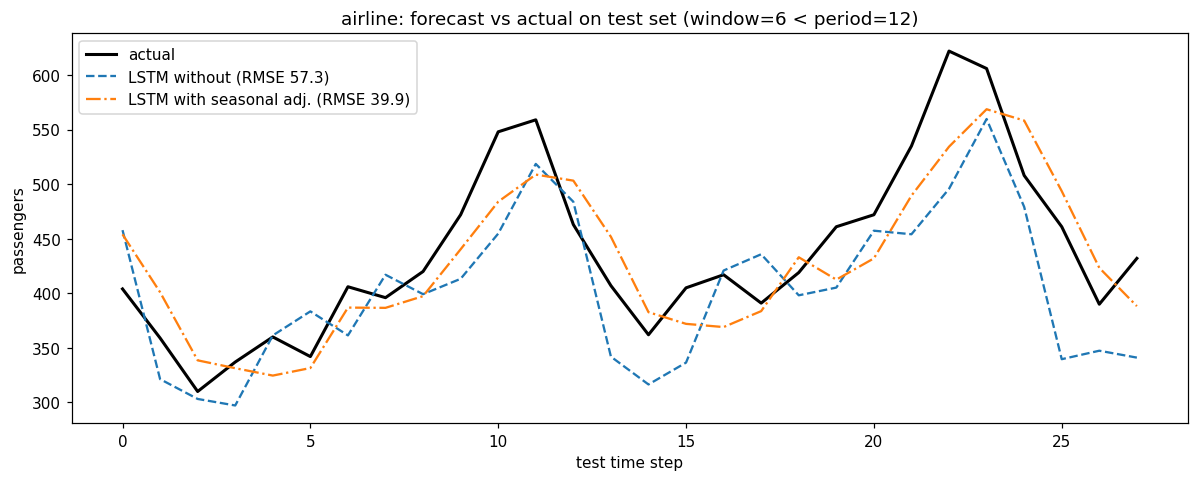
\includegraphics[width=0.9\textwidth]{seasonality_outputs/airline_seasonality_forecast.png}
    \caption{Airline: So sánh dự báo LSTM có/không điều chỉnh mùa vụ ($n\_steps=6 <$ period=12)}
\end{figure}

% ============================================================
\section{Câu hỏi Phản ánh}

\subsection*{1. Tại sao không được xáo trộn chuỗi thời gian trước khi chia tập?}

Chuỗi thời gian có cấu trúc phụ thuộc nhân quả: $x_t$ phụ thuộc $x_{t-1}, x_{t-2},\ldots$ Nếu xáo trộn, một mẫu train có thể chứa $(x_{100}, x_{101}, x_{102})$ trong khi mẫu liền kề trong test là $(x_{98}, x_{99}, x_{100})$ --- mô hình đã thấy $x_{102}$ trước khi ``dự đoán'' $x_{100}$. Thông tin từ tương lai rò rỉ vào huấn luyện. Kết quả đánh giá sẽ \textit{optimistically biased} và không phản ánh khả năng dự báo thực tế.

\subsection*{2. MLP xử lý window như vector phẳng nhưng vẫn tốt --- điều này nói lên gì?}

Phần lớn thông tin dự báo nằm ở \textit{độ lớn} (magnitude) của các giá trị trong cửa sổ, không phải ở thứ tự chính xác của chúng. Biết ``đã ở đâu gần đây'' quan trọng hơn biết ``trình tự cụ thể''. Thứ tự thực sự quan trọng khi cần nắm bắt phụ thuộc dài hạn, mẫu phi tuyến phức tạp, hoặc asymmetry (tăng nhanh/giảm chậm) --- đó là khi LSTM vượt trội MLP.

\subsection*{3. Khi nào CNN tốt hơn MLP? Khi nào LSTM đáng chi phí?}

\textbf{CNN hơn MLP khi:} chuỗi có các mẫu cục bộ lặp lại (đột biến, đỉnh, đoạn cong đặc trưng) mà convolution kernel có thể phát hiện; dữ liệu nhiều nhiễu (pooling layer lấy đặc trưng bền vững hơn).

\textbf{LSTM đáng chi phí khi:} cần phụ thuộc dài hạn mà cửa sổ cố định không nắm được (ví dụ: pattern xảy ra sau hàng trăm bước); chuỗi có cấu trúc ngữ nghĩa nơi \textit{thứ tự} thực sự mang thông tin (ngôn ngữ tự nhiên, chuỗi sự kiện).

\subsection*{4. Tại sao RMSE không có baseline là vô nghĩa?}

Không có ngữ cảnh, không có con số nào có giá trị. ``RMSE = 21.3 nghìn hành khách'' --- tốt hay xấu? Chỉ khi biết baseline = 53.4 mới thấy mô hình tốt hơn $60\%$. Mức tối thiểu cần báo cáo: (1) Naive baseline RMSE, (2) Model RMSE trong đơn vị thực, (3) \% cải thiện. Baseline trả lời câu hỏi: ``Giải pháp ngốc nghếch nhất đạt được gì?'' --- nếu mô hình không vượt được câu trả lời đó, toàn bộ công sức tối ưu kiến trúc là vô ích.

\subsection*{5. Tại sao sai số multi-step tăng theo horizon?}

Hai lý do chính:
\begin{enumerate}
    \item \textbf{Thông tin suy giảm theo khoảng cách:} Tương quan giữa $x_t$ và $x_{t+k}$ giảm theo $k$. Tại horizon xa, cửa sổ hiện tại ngày càng ít liên quan.
    \item \textbf{Bất định tích lũy:} Mỗi bước tiếp theo trong tương lai có thêm một biến ngẫu nhiên $\epsilon_{t+k}$. Entropy dự báo tăng đơn điệu --- đây là giới hạn lý thuyết không thể vượt qua, không phải lỗi của mô hình.
\end{enumerate}

\subsection*{6. Neural networks tha thứ cho non-stationarity hơn ARIMA --- tại sao?}

ARIMA giả định tường minh rằng chuỗi dừng; nếu vi phạm, ước lượng tham số bị sai lệch và dự báo phân kỳ. Neural networks không có giả định này --- chúng học hàm ánh xạ $f(x_{t-n},\ldots,x_{t-1}) \to x_t$ trực tiếp từ dữ liệu. Với đủ dữ liệu, mạng có thể học ngầm định cả xu hướng và mùa vụ mà không cần dừng hóa tường minh.

\textbf{Khi nào vẫn nên làm sai phân cho neural network:}
\begin{itemize}
    \item Xu hướng rất mạnh gây gradient lớn, làm mất ổn định huấn luyện.
    \item Muốn cải thiện tốc độ hội tụ (sai phân thu hẹp phạm vi giá trị, scaling hiệu quả hơn).
    \item Kết hợp với ARIMA dạng hybrid: ARIMA xử lý phần linear, neural network học phần nonlinear còn lại.
\end{itemize}

% ============================================================
\section*{Kết luận}

Qua bài thực hành này, các kỹ năng cốt lõi đã được xây dựng:

\begin{enumerate}
    \item \textbf{Sliding window} --- chuyển đổi chuỗi thời gian thành bài toán học có giám sát $(X, y)$, cả one-step và multi-step.
    \item \textbf{MLP, CNN, LSTM} --- xây dựng, huấn luyện và đánh giá ba kiến trúc cơ bản, hiểu điểm mạnh của từng loại.
    \item \textbf{Preprocessing đúng cách} --- chronological split, leak-free scaling, inverse-transform để đảm bảo đánh giá không bị sai lệch.
    \item \textbf{Naive baseline} --- bài học quan trọng nhất: trên temps, chỉ LSTM vượt được baseline đơn giản; MLP và CNN thậm chí kém hơn. RMSE mà không có baseline là con số trống rỗng.
    \item \textbf{Window size} --- $n\_steps \approx$ chu kỳ mùa vụ là điểm xuất phát tốt; PACF là công cụ hữu ích để dự đoán trước khi thực nghiệm.
    \item \textbf{Seasonal adjustment} --- có ích khi cửa sổ ngắn hơn chu kỳ, phản tác dụng khi cửa sổ đủ dài để mô hình tự học.
\end{enumerate}

\end{document}
